\section{Introduction}

\begin{figure}[!t]
  \centering
  \begin{subfigure}{0.55\linewidth}
    \centering
    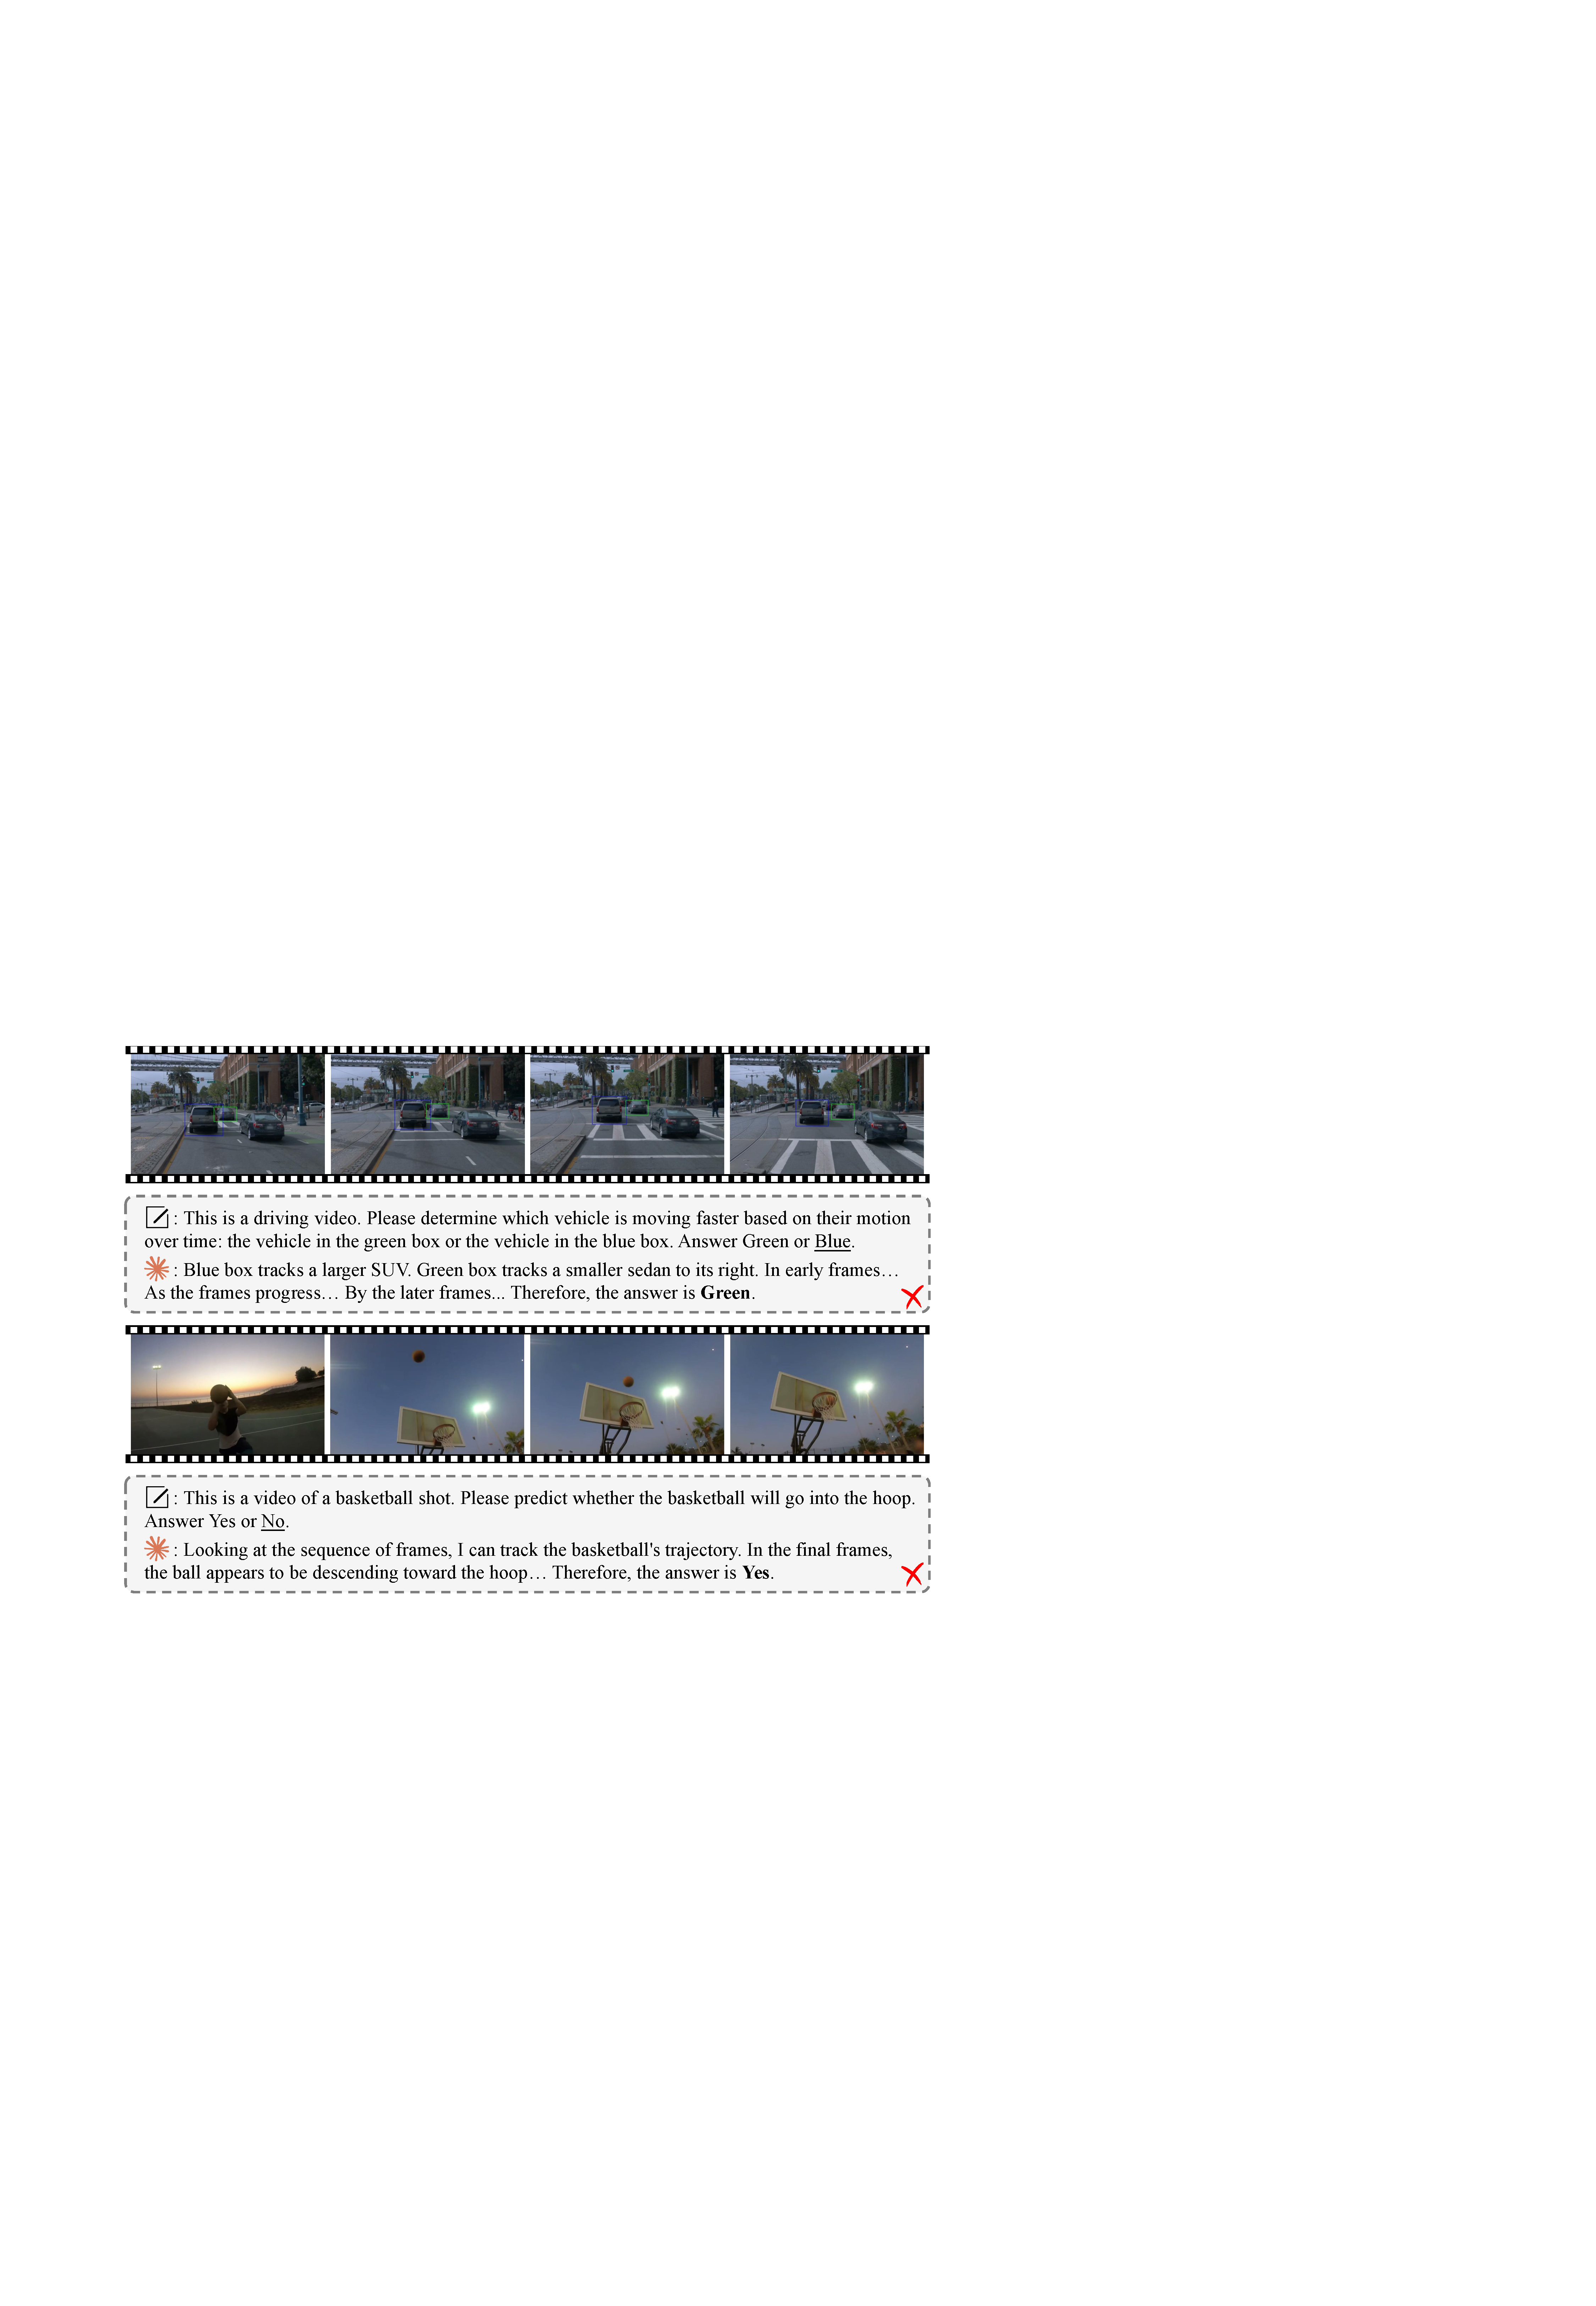
\includegraphics[height=0.25\textheight]{fig/fig_1_a.pdf}
    \caption{}
    \label{fig:1a}
  \end{subfigure}
  \begin{subfigure}{0.35\linewidth}
    \centering
    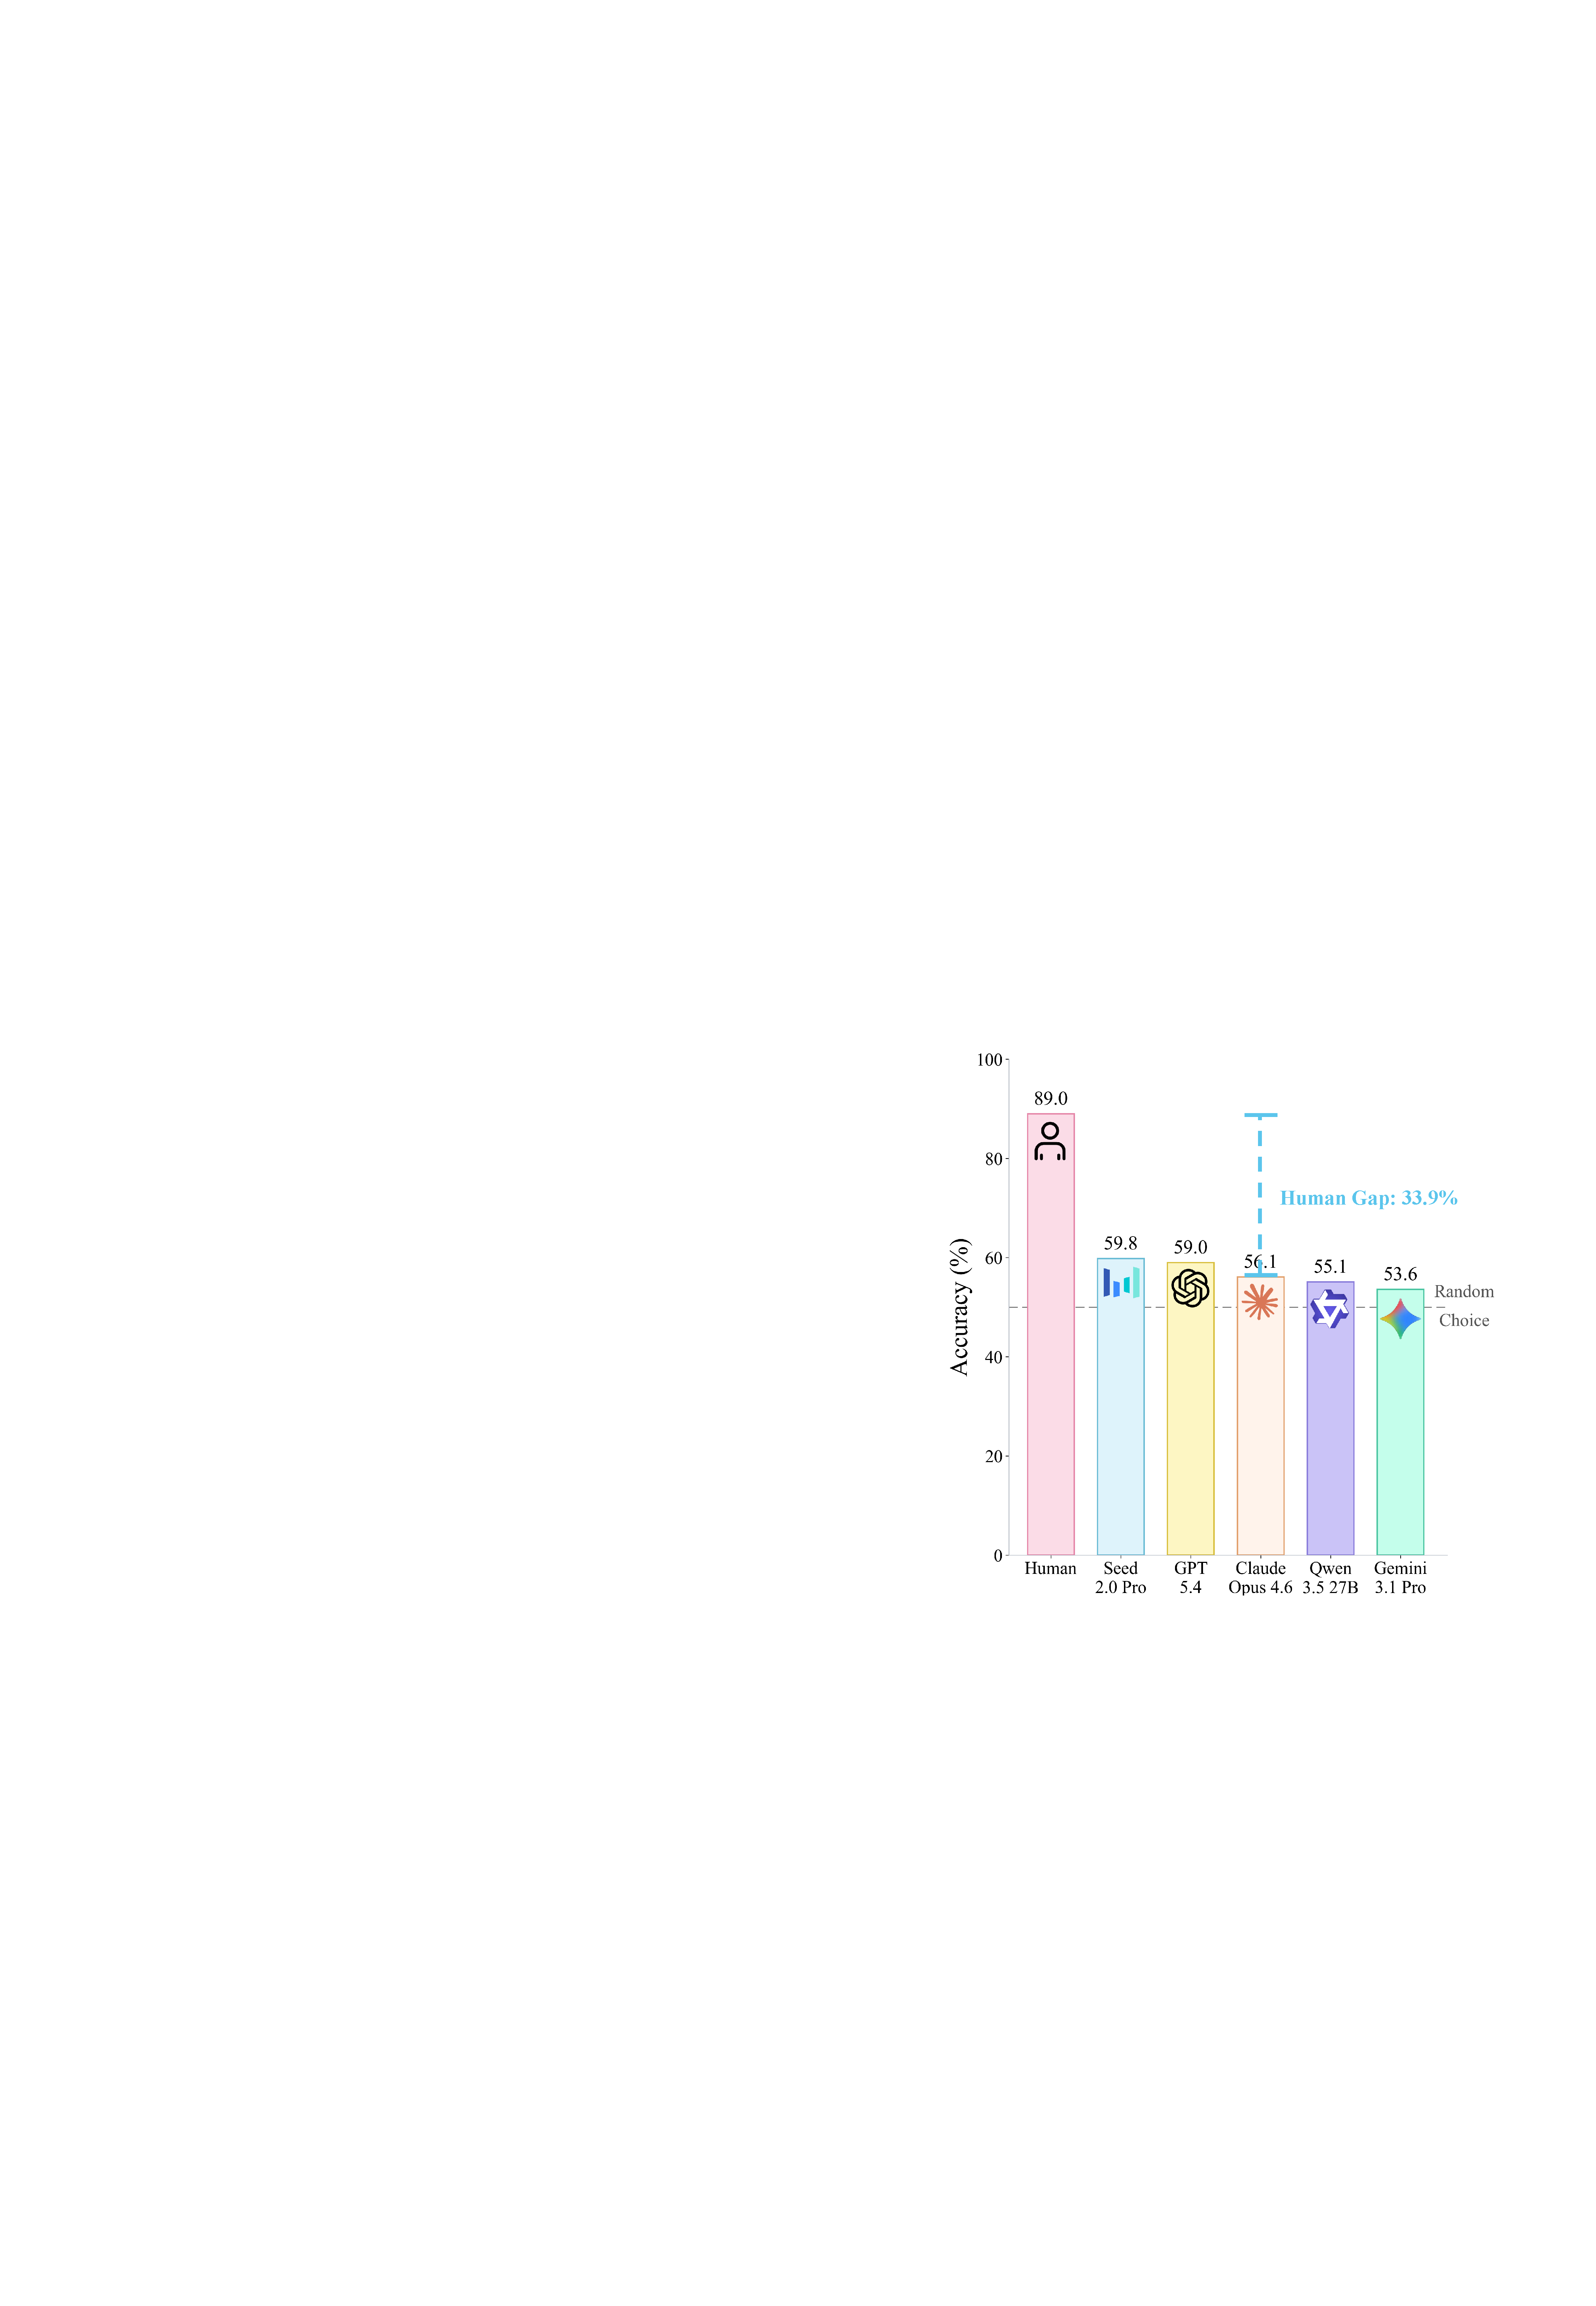
\includegraphics[height=0.25\textheight]{fig/fig_1_b.pdf}
    \caption{}
    \label{fig:1b}
  \end{subfigure}
  \caption{\textbf{Motivating examples and benchmark results.} (a) Two representative examples from ViSTR-Bench, where underlined options indicate the correct answers. Although these questions are visually straightforward for humans, Claude~\citep{Claude} still produces incorrect answers, highlighting the difficulty of reasoning from continuous visual cues in dynamic scenes. (b) Quantitative evaluation results on ViSTR-Bench, showing that current MLLMs remain far from human-level spatial-temporal reasoning performance.}
  \label{fig:1}
\end{figure}

% In recent years, Multimodal Large Language Models (MLLMs) have demonstrated remarkable proficiency across diverse domains, ranging from complex analytical tasks such as mathematical reasoning~\citep{MathVista,MATH-Vision,MATHVERSE} and programming~\citep{MMCode,Design2Code} to high-quality visual content generation~\citep{Emu3,NExT-GPT,MiniGPT-5}. 
% However, a significant gap remains between these capabilities and the physical intelligence required to reason about the real world. MLLMs still struggle with fundamental abilities that humans naturally acquire through continuous observation and interaction with the environment, including spatial perception, temporal awareness, and dynamic reasoning. 
% Such spatial-temporal reasoning capabilities are indispensable for real-world applications, including autonomous driving~\citep{LMDrive,DriveLM,DriveGPT4}, robotics~\citep{OpenVLA,RT-2}, and embodied AI~\citep{SayCan,PaLM-E}.

In recent years, Multimodal Large Language Models (MLLMs) have demonstrated remarkable proficiency across diverse domains, ranging from complex analytical tasks such as mathematical reasoning~\citep{MathVista,MATH-Vision,MATHVERSE} and programming~\citep{MMCode,Design2Code} to high-quality visual content generation~\citep{Emu3,NExT-GPT,MiniGPT-5}. 
For example, GPT-5 Pro~\citep{GPT-5} achieved 88.4\% accuracy on GPQA~\citep{GPQA}, a PhD-level scientific reasoning benchmark on which human experts achieve only 65.0\% accuracy.
However, despite these expert-level capabilities, which typically require long-term specialized training for humans to acquire, MLLMs still struggle with fundamental abilities that humans naturally develop through continuous observation and interaction with the environment, including spatial perception, temporal awareness, and dynamic reasoning, as illustrated in Figure~\ref{fig:1a}.
These spatial-temporal reasoning capabilities are indispensable for real-world applications such as autonomous driving~\citep{LMDrive,DriveLM,DriveGPT4}, robotics~\citep{OpenVLA,RT-2}, and embodied AI~\citep{SayCan,PaLM-E}.

While recent efforts have recognized this gap and introduced benchmarks to evaluate the visual spatial intelligence of MLLMs, several critical limitations remain in current task designs. 
First, existing evaluations~\citep{OmniSpatial,MMSI-Video-Bench,SpaceR,VSI-Bench,Cambrian-S,SPAR-Bench} predominantly focus on static spatial attributes, such as object scale and scene geometry, while largely neglecting the modeling of continuous temporal information. 
Second, although some benchmarks incorporate dynamic scenes~\citep{Dyn-Bench,STI-Bench,OST-Bench,VideoLoom,MLLM-4D,DSI-Bench,DSR-Bench,VLM4D}, their tasks are often restricted to low-level perception, such as object counting or trajectory tracking, falling short of the high-level reasoning needed to infer future states beyond immediate observations. 
Third, many tasks~\citep{STI-Bench,VideoLoom,MLLM-4D,DSR-Bench} rely on quantitative evaluation, which may conflate numerical prediction accuracy with genuine spatial-temporal reasoning ability.

To address these limitations, we introduce the \textbf{Vi}sual \textbf{S}patial-\textbf{T}emporal \textbf{R}easoning \textbf{Bench}mark (\textbf{ViSTR-Bench}), designed to systematically evaluate whether MLLMs can reason from continuous visual cues in dynamic scenes. 
Guided by three core principles, namely \textit{temporal emphasis}, \textit{reasoning orientation}, and \textit{qualitative evaluation}, ViSTR-Bench is structured around four task dimensions:
(1) \textbf{Motion Perception} evaluates whether models can identify and compare object motion over time, especially under ego-motion and environmental distractors;
(2) \textbf{Spatial Relations} requires models to reason about evolving geometric relationships and spatial constraints, such as observer-object relations under camera motion and collision-free passage feasibility;
(3) \textbf{Outcome Prediction} assesses the ability to infer current motion states from historical cues and anticipate future outcomes before they are directly observed; 
(4) \textbf{Physical Dynamics} focuses on intrinsic physical properties, dependencies, and stability conditions that are ambiguous in static images but become evident through dynamic interactions.

Specifically, ViSTR-Bench consists of 12 subtasks and 1,093 high-quality video question-answer pairs, spanning tabletop, indoor, and outdoor scenes. The data are collected from multiple sources, including public datasets (e.g., Ego4D~\citep{Ego4D}, ScanNet~\citep{ScanNet}, ScanNet++~\citep{ScanNet++}, ARKitScenes~\citep{ARKitScenes}, and Waymo~\citep{Waymo}), web videos, and self-collected recordings. 
We conduct extensive evaluations on a diverse set of advanced MLLMs, including proprietary general-purpose MLLMs (e.g., GPT~\citep{GPT-5}, Gemini~\citep{Gemini}, and Claude~\citep{Claude}), open-source general-purpose MLLMs (e.g., Qwen~\citep{Qwen3.5} and InternVL~\citep{InternVL3.5}), and specialized spatial MLLMs (e.g., Spatial-MLLM~\citep{Spatial-MLLM}, Spatial-SSRL~\citep{Spatial-SSRL}, and GeoThinker~\citep{GeoThinker}). As shown in Figure~\ref{fig:1b}, experimental results demonstrate that, despite the impressive progress of current MLLMs in general video question answering, they still exhibit substantial bottlenecks in tasks that require subtle motion perception, complex relational reasoning, and temporal cue modeling, with a considerable gap remaining compared to human performance.

Our main contributions are summarized as follows:
\begin{itemize}
\item We introduce the \textbf{Vi}sual \textbf{S}patial-\textbf{T}emporal \textbf{R}easoning \textbf{Bench}mark (\textbf{ViSTR-Bench}) to systematically evaluate whether MLLMs can perform qualitative spatial-temporal reasoning from continuous visual cues in dynamic scenes.

\item We establish a four-dimensional evaluation framework covering Motion Perception, Spatial Relations, Outcome Prediction, and Physical Dynamics, and construct a benchmark comprising 12 diverse subtasks and 1,093 high-quality video question-answer pairs across tabletop, indoor, and outdoor scenarios.

\item We conduct comprehensive evaluations on a broad range of advanced MLLMs, revealing that current models, despite their progress in general video question answering, still fall substantially short of human performance when understanding dynamic physical scenes.
\end{itemize}
